\documentclass[a4paper,12pt]{report}

\usepackage{alltt, fancyvrb, url}
\usepackage{graphicx}
\usepackage[utf8]{inputenc}
\usepackage{float}
\usepackage{hyperref}

% Questo commentalo se vuoi scrivere in inglese.
\usepackage[italian]{babel}

\usepackage[italian]{cleveref}

\title{Relazione \\``Time2Survive''}

\author{Andrea Cecchini \\ Nicolò D'Addabbo \\ Luca Oskari Fiumanò \\Leonardo David Matteo Magnani}
\date{\today}


\begin{document}

\maketitle

\tableofcontents

\chapter{Analisi}

\section{Requisiti}
Il progetto si pone l’obiettivo di creare un videogioco survival shoot ‘em up ispirato a ``The Binding of Isaac'' \footnote{\url{https://store.steampowered.com/app/113200/The_Binding_of_Isaac/}}.
Con survival shoot ‘em up si intende un genere di videogioco nella quale l’obiettivo è sopravvivere il più a lungo possibile a ondate di nemici, generandone di nuove una volta eliminata la precedente.

\subsection*{Requisiti funzionali}
\subsubsection{Requisiti Funzionali Obbligatori}
\begin{itemize}
	\item Il gioco dovrà occuparsi di gestire la partita dell’utente all’interno della mappa di gioco di Time2Survive, rendendo più difficile la sopravvivenza del giocatore attraverso ondate di nemici di difficoltà crescente.
    All’interno della mappa, il giocatore potrà:
    \begin{itemize}
        \item Sfruttare le proprie abilita’ di videogiocatore per sopravvivere alle numerose ondate dei nemici che si susseguiranno.
        \item Sfidare ondate che verranno generate al completamento della precedente. Le ondate terminano quando tutti i nemici sono stati eliminati.
        \item I nemici si potranno eliminare attraverso l'utilizzo di proiettili generati dal personaggio.
        \item La partita sarà conclusa alla morte virtuale del giocatore.
    \end{itemize}
	\item Il giocatore si troverà all'interno di una stanza in cui verranno generate le ondate di nemici.
	\item La difficoltà del gioco sarà incrementale e riguarderà sopratutto le ondate. Essa sarà manipolata attraverso 3 parametri:
    \begin{itemize}
        \item Numero: numero dei nemici a schermo.
        \item Resilienza: resistenza agli attacchi da parte del giocatore.
        \item Forza: danno provocato dal nemico.
    \end{itemize}
	\item Il giocatore si potrà muovere nell’ambiente di gioco costituito da una singola stanza.
    \item I nemici sono delle entità attive del gioco che cercano di eliminare il giocatore.
    Vengono controllati da una semplice AI (Artificial Intelligence). 
	Per intelligenza artificiale si intende un software che conferisce a ogni nemico una strategia di movimento e di combattimento.
    \item Il giocatore dovrà essere in grado di capire lo stato della partita in ogni momento della suddetta visualizzando la propria vita. 
	Il giocatore sarà inoltre in grado di visualizzare le proprie capacità essendo in grado di visualizzare il numero di ondate alle quali è sopravvissuto.
\end{itemize}

\subsubsection{Requisiti Funzionali Opzionali}
\begin{itemize}
	\item Per aiutare il giocatore, saranno disponibili diversi potenziamenti che gli permetteranno di aumentare le proprie abilità.
	\item Per rendere più vario la partita saranno presenti diversi tipi di nemici con caratteristiche uniche e diverse tra loro.
\end{itemize}
\subsection*{Requisiti non funzionali}
\begin{itemize}
	\item Il programma deve mantenere un profilo di prestazione adeguato e costante nonostante il variare dello stato del mondo di gioco alla fine di garantire un’esperienza di gioco fluida e gradevole.
	\item Per rendere il videogioco il più godibile possibile la grafica dovrà essere elaborata con uno stile grafico al passo coi tempi.
\end{itemize}
\newpage
\section{Analisi e modello del dominio}
T2S mette a disposizione del giocatore la possibilità di giocare una nuova partita, che gestirà lo stato e il mondo di gioco.
\\
Il mondo di T2S è l’arena dove le diverse entità interagiscono fra di loro.
\\
Al giocatore sarà data la possibilità di controllare una di queste entità che rappresenterà il giocatore all’interno della partita.
\\
Durante lo svolgimento della partita verranno generate delle ondate di entità controllate da un’intelligenza artificiale con il compito di attaccare e uccidere il giocatore.
Per combattere questi nemici, il giocatore avrà la possibilità di sparare dei proiettili e di ottenere diversi tipi di power up, durante round prestabiliti e continui, 
che renderanno il più semplice sconfiggere tutti i nemici che gli si porranno avanti.
Una volta sconfitta un’ondata viene aggiornato lo stato della partita incrementando il numero di round alla quale si è sopravvissuti 
e generandone una nuova di maggiore difficoltà.
All’inizio della partita all’avatar verranno assegnati dei proiettili di default e un determinato numero di punti vita.
Una volta subito un danno, a seconda della sua entità, verrà detratta una certa quantità dalla vita corrente, una volta persa tutta il gioco terminerà mostrando 
al giocatore per quanto è sopravvissuto.
Le difficoltà che il progetto si porta dietro sono:
\begin{itemize}
	\item Un’implementazione di un intelligenza artificiale in grado di controllare correttamente i nemici.
	La prima versione del gioco fornirà ai nemici un Controller basato sulle coordinate del player nella mappa.
	\item Una grafica completa che verrà implementata inizialmente in maniera minimale.
\end{itemize}

\begin{figure}[H]
\centering{}
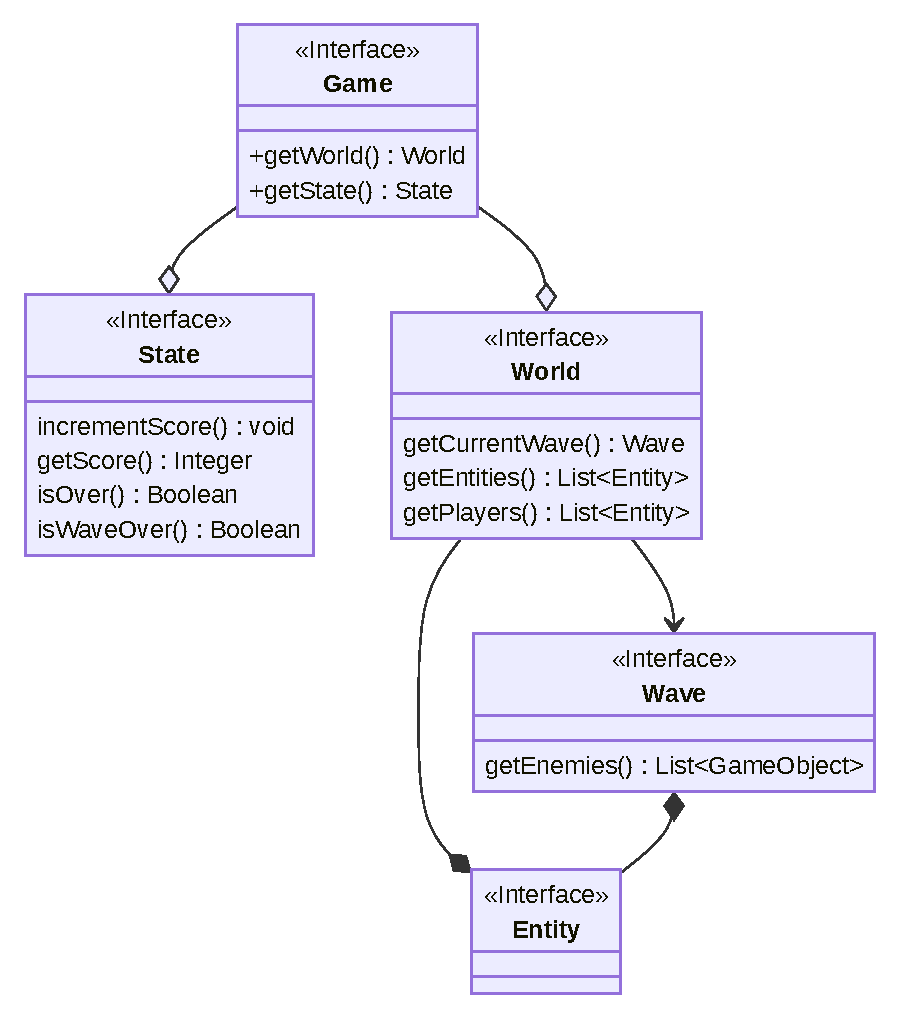
\includegraphics[width=1\textwidth]{img/AnalysisDomainUML-1.pdf}
\caption{Schema UML dell'analisi del problema, con rappresentate le entità principali ed i rapporti fra loro}
\label{img:analysis}
\end{figure}




\chapter{Design}
\section{Architettura}
T2S è stato sviluppato adottando un pattern architetturale che mantenesse una simile struttura MVC, quindi con i suoi vantaggi, contaminandola però attraverso l’utilizzo del pattern Component.
\\
Il pattern Component permette a una singola entità di estendersi su domini multipli senza accorparli in unica classe.
\\
Applicandolo al dominio dell’applicazione (Model), avremo che ogni entità risulta essere un entità di gioco denominata Entity.
Tale Entity verrà adornato da dei Component, ognuno dei quali appartiene a un dominio particolare (Input, Fisica, Grafica, …), che è sarà responsabile dell’aggiornamento del dominio all’interno dell’Entity.
Tuttavia, pur appartenendo a domini diversi, i diversi componenti potrebbero aver bisogno di comunicare tra di loro.
Sfruttando come “container” l’Entity stesso è stato messo a disposizione ai Components un semplice ma funzionale sistema di messaggistica.
L’utilizzo di questi componenti porta ad importanti vantaggi:
\begin{itemize}
	\item \textbf{Stroncamento di un albero di ereditarietà troppo complesso e lungo}:
	Per rappresentare entità con diversi comportamenti si utilizza la composizione di GameComponent che implementino quei comportamenti, senza nessun utilizzo dell’ereditarietà.
	%
	\item Eliminazione dei problemi legati all’ereditarietà multipla
	%
	\item \textbf{Riduzione al minimo delle ripetizioni di codice} dovuto alla creazione di componenti altamente riutilizzabili
\end{itemize}
Dal punto di vista del pattern architetturale Model-View-Controller, i rispettivi moduli sono rappresentati da:
\begin{itemize}
	\item \textbf{Model}:
	Il ruolo del "Model" viene affidato all'insieme delle classi che sono contenute nella classe Game (inclusa).
	Difatti, se per creare un gioco diverso da T2S basterebbe cambiare la parte di "Model" dell'architettura in questione, le parti da sostituire ricadono nell'insieme sopra citato.
	\item \textbf{Controller}:
	Questo ruolo viene affidato all’interfaccia GameEngine, la quale ha il compito di gestire l’aggiornamento di ogni Entity, dei suoi componenti e della sua renderizzazione sulla View.
	\item \textbf{View}:
	Il ruolo della view viene demandato a delle interfacce ben connesse tra di loro: GameScene e Graphics.
	L’interfaccia GameScene astrae il concetto di “Scena” di gioco
	L’interfaccia Graphics ha il compito di saper “disegnare” le diverse entità con la 
	tecnologia grafica che si è scelto di utilizzare.
\end{itemize}
Dal diagramma delle classi, qui sotto fornito, è possibile notare un elemento di differenza rispetto a una classica architettura MVC: un componente di spicco, denominato GraphicsComponent, risulta avere dei riferimenti alla parte di view e di model, creando un collegamento che a prima vista potrebbe risultare problematico.
La modularità di M.V.C. non viene però attaccata: volendo, come esempio, cambiare la tecnologia di sviluppo per quanto riguarda la grafica si modificherà esclusivamente la parte di View dell'applicazione, senza ripercussioni in nessun altro modulo del programma.
L’ipotetico passaggio da JavaFX a Swing o ad altre tecnologie, dunque, non risulta essere problematico: 
si dovranno sostituire le implementazioni di JavaFX delle interfacce Graphics, GameScenecon delle nuove implementazioni che utilizzino la nuova tecnologia.
	
\begin{figure}[H]
\centering{}
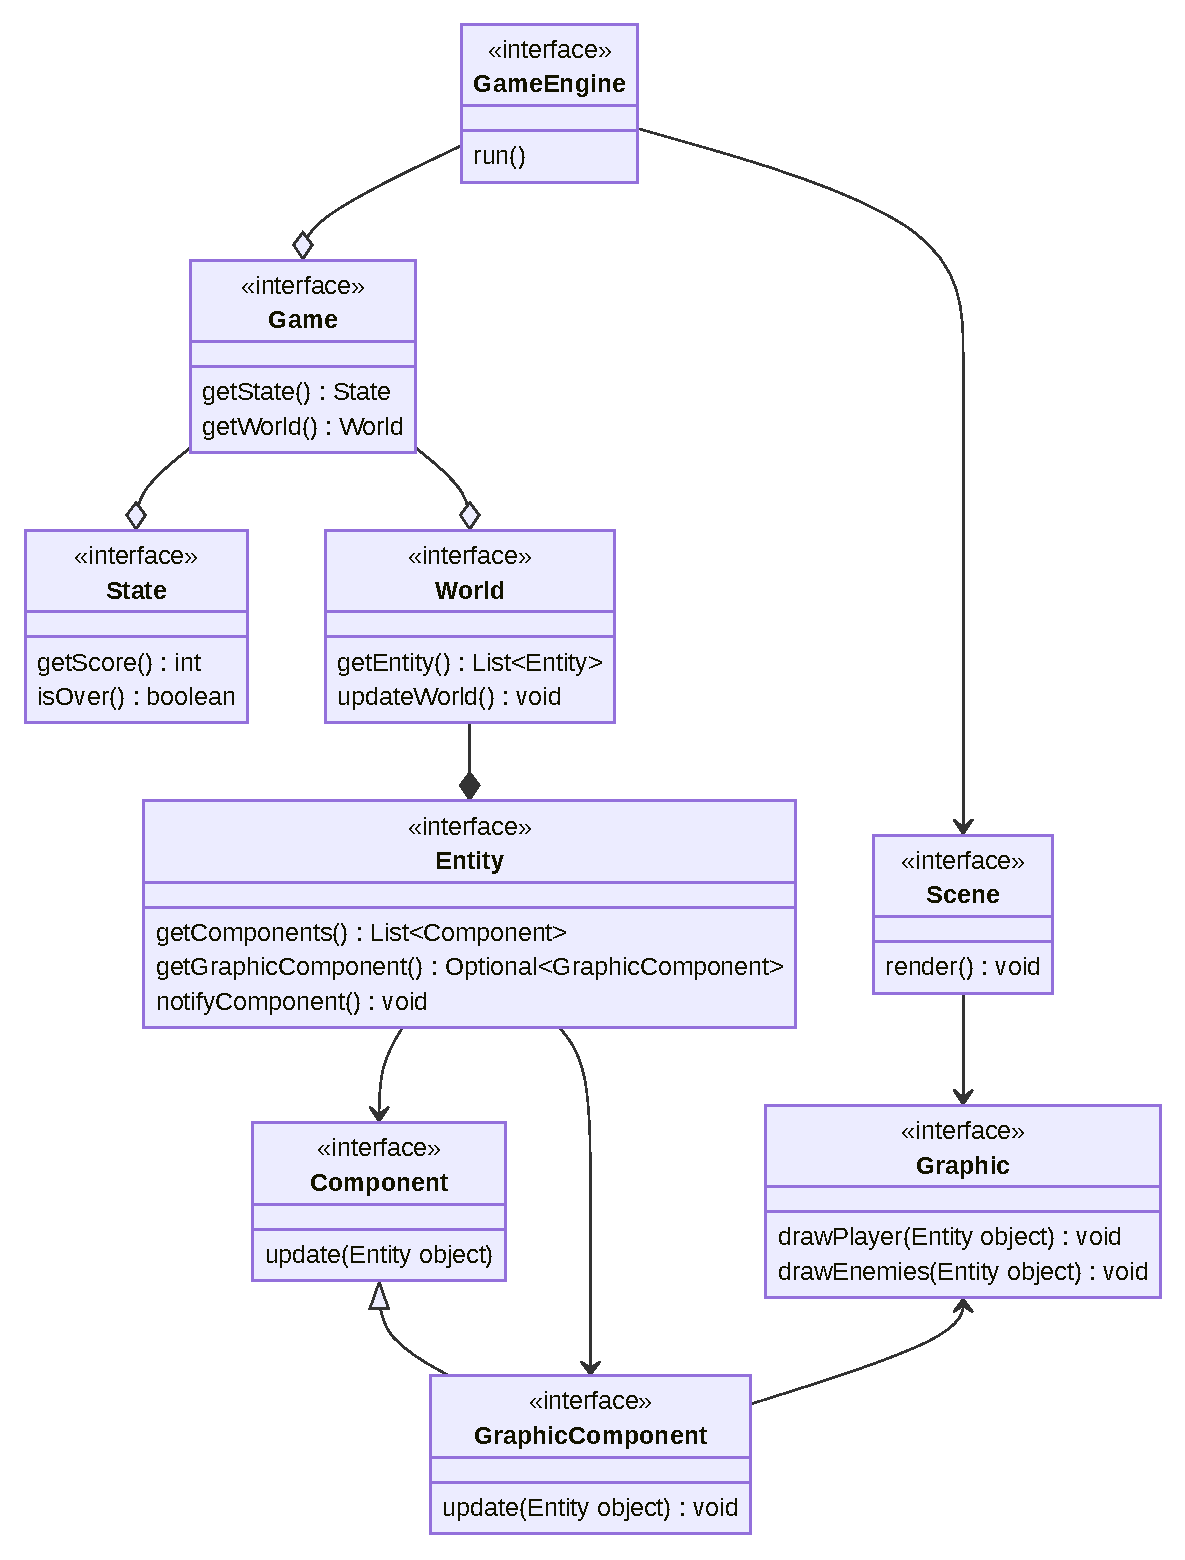
\includegraphics[width=1\textwidth]{img/SoftwareArchitectureUML.pdf}
\caption{Schema UML architetturale di T2S.}
\label{img:analysis}
\end{figure}

\section{Design dettagliato}
%
\subsection*{Cecchini Andrea}
%
\subsubsection*{Separare il dominio del GameLoop da quello del GameEngine}
%
\begin{figure}[H]
	\centering{}
	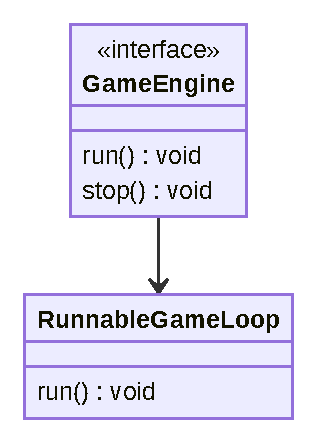
\includegraphics[scale=0.75]{img/GameEngineAndGameLoop.pdf}
	\caption{Rappresentazione UML del pattern Strategy per separare il dominio della classe GameLoop da quello del GameEngine.}
	\label{img:strategy}
	\end{figure}
%
\paragraph*{Problema} Disacoppiare la logica della classe \textbf{GameLoop} dal logica della classe \textbf{GameEngine}, al fine di garantire il \textbf{Single Responsability Principle}.
%
\paragraph*{Soluzione} La classe GameEngine utilizza il pattern \textbf{Strategy} al fine di delegare alla classe \textbf{RunnableGameLoop} la gestione del dominio del GameLoop. 
Quindi, alla classe GameEngine avrà la responsabilità di gestire solamente ciò che le compete, delegando il resto.
%
\subsubsection*{Decorazione della classe GameLoop}
%
\begin{figure}[H]
	\centering{}
	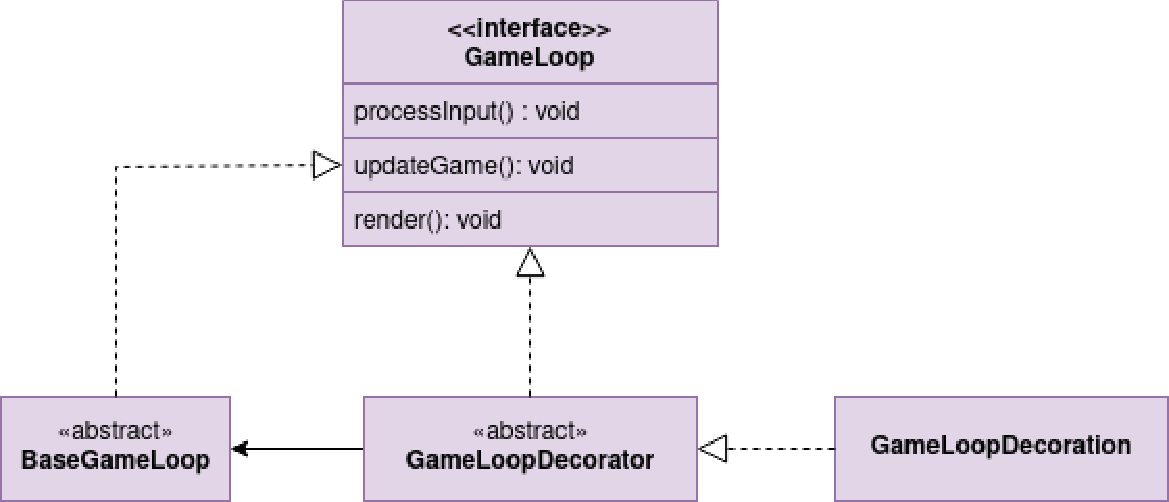
\includegraphics[scale=0.75]{img/GameLoopDecorator.pdf}
	\caption{Rappresentazione UML del Decorator pattern per il GameLoop}
	\label{img:strategy}
	\end{figure}
%	
\paragraph*{Problema} La classe \textbf{GameLoop} risulta essere prona alla confusione e alla non manutibilità.
Questo è dovuto alla natura stessa del GameLoop, nel quale al suo interno si sviluppano diversi domini e logiche quali:
\begin{itemize}
	\item Processione dell'input.
	\item Aggiornamento dello stato di gioco
	\item Gestione della renderizzazione.
\end{itemize}
Inoltre, ognuno di questi domini potrebbe raccogliere delle particolarità che possono differire dalla implementazione basica contenuta in \textbf{BaseGameLoop}.
Aggiungere nuove feature risulta quindi essere un lavoro poco gradevole e prono alla aggiunti di possibili errori.
%
\paragraph*{Soluzione} Utilizzare il pattern \textbf{Decorator}, nel quale il BaseGameLoop viene decorato con delle possibili implementazioni di decorazione, permette di risolvere tutti i problemi sopra presentati:
\\
In particolare il codice non risulta piu' essere accumulato in un punto specifico della classe BaseGameLoop e 
l'aggiunta di nuove feature, riguardante i domini sopra citati, risulta essere estremamente facile, difatti basta aggiungere una nuova decorazione al game loop già sviluppato.
\\
Il codice risulta essere estremamente manutenibile, questo dovuto alla separazione di codice che il pattern Decorator offre.
%
\subsubsection*{Implementare diversi tipi di basi per il game loop}
%
\begin{figure}[H]
	\centering{}
	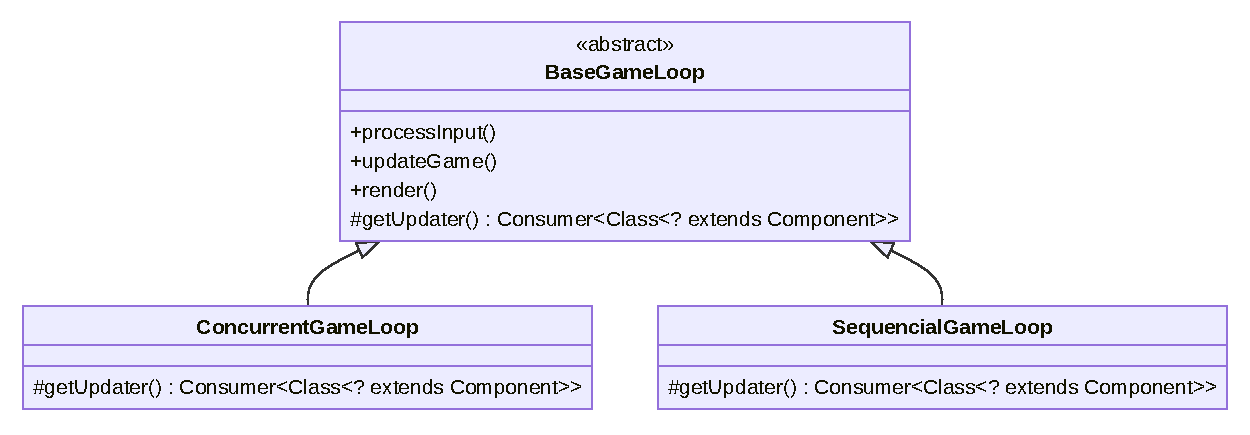
\includegraphics[scale=0.75]{img/TemplateMethodOnBaseGameLoop.pdf}
	\caption{Rappresentazione UML del pattern Template Method per la creazione di GameLoops Base}
	\label{img:strategy}
	\end{figure}
%
\paragraph*{Problema} Esistono due versioni di BaseGameLoop, una nel quale i componenti vengono aggiornati parallelamente e un'altra sequenzialmente.
Ci si è accorti che le due implementazioni condividevano gran parte del codice, avendo quindi una ripetizione.
%
\paragraph*{Soluzione} Essendo che le due implementazioni differiscono solo per il tipo di updater, è stato utilizzato il \textbf{Template Method} al fine di massimizzare il riuso.
I metodi template sono \texttt{processInput()}, \texttt{updateGame()}, \texttt{render()}, che chiamano un metodo astratto e protetto \texttt{getUpdater()}. 
%
\subsubsection*{Gestione delle collisioni fra figure di forma diverse}
%
\begin{figure}[H]
	\centering{}
	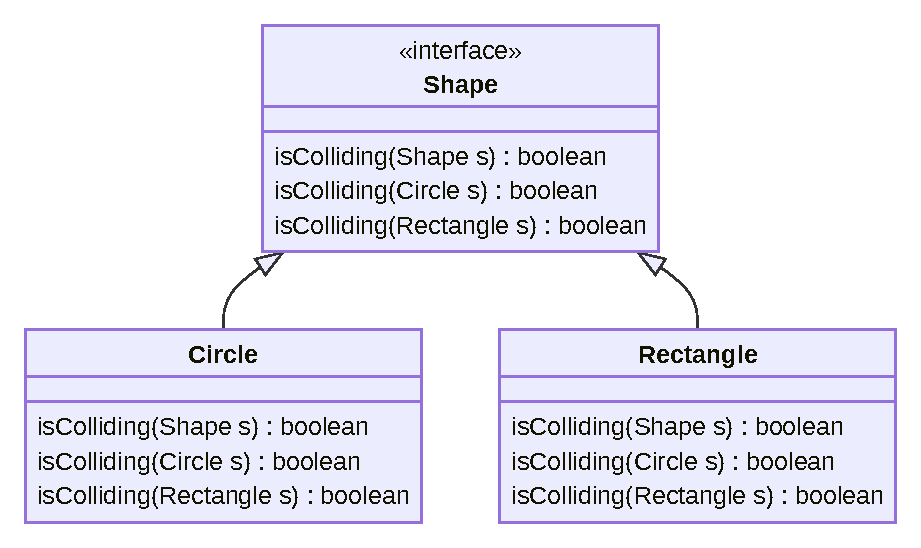
\includegraphics[scale=0.75]{img/VisitorPattern.pdf}
	\caption{Rappresentazione UML del pattern Visitor Pattern per la gestione delle collisioni con figure di forma diversa.}
	\label{img:strategy}
	\end{figure}
%
\paragraph*{Problema} L'istanza della classe \textbf{Shape} ha bisogno di sapere l'implementazione della figura della quale sta verificando la possibili collisione, al fine di addattare i propri calcoli verificare se vi è stata o meno la collisione con quella figura. 
%
\paragraph*{Soluzione} La soluzione scelta rispetta l'implementazione del pattern \textbf{Visitor}.
Tale implementazione suggerisce di delegare alla Shape \textbf{s} il controllo della collisione con la Shape \textbf{this}.
Questa soluzione permette rende possibile aggiunta di nuove figure in modo facile, senza dover creare un costrutto switch o if-else al fine di controllare la reale implementazione della shape s.
%%

\subsection*{Nicolò D'Addabbo}

\subsubsection{Input Controller intercambiabili}

\begin{figure}[H]
\centering{}
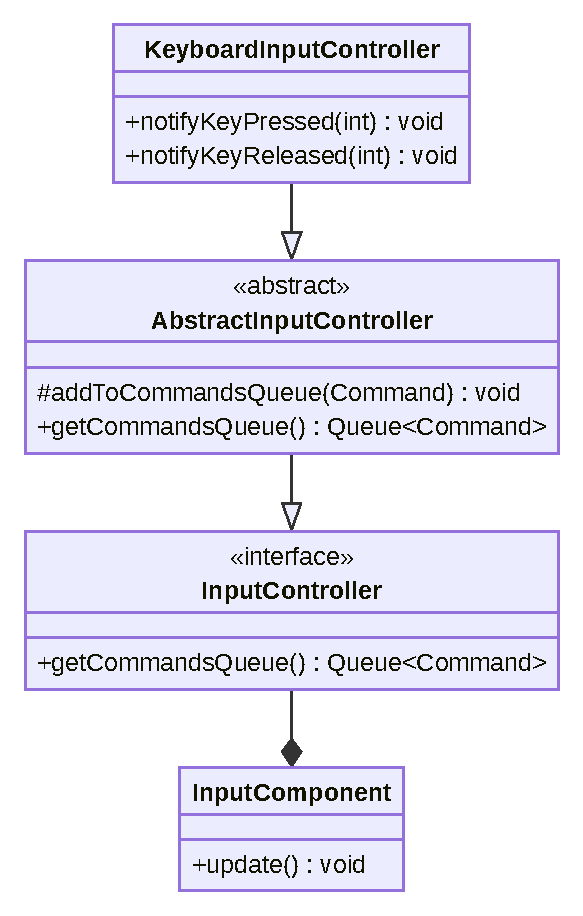
\includegraphics[scale=0.75]{img/InputControllerUML}
\caption{Rappresentazione UML del pattern Strategy per l'Input Component}
\label{img:strategy}
\end{figure}

\paragraph{Problema} Un’entità può ricevere input da diverse sorgenti come ad esempio una tastiera o un joypad, 
la cui presenza non è di interesse dell’entità stessa. 
Infatti deve possedere solo un generico Input Component con un metodo update.

\paragraph{Soluzione} La classe \textbf{InputComponent} implementa lo \textit{Strategy pattern}, contenendo un riferimento a un \textit{InputController} che funge da strategia per la gestione dell'input. Quest'ultimo può essere sostituito con un'implementazione diversa, permettendo l'utilizzo di strategie differenti.
\\
Il metodo \textit{update} dell’Input Component chiama il metodo \textit{execute} su ogni \textit{Command} (come descritto nella sezione "Gestione dei comandi di gioco") presente nella coda di comandi restituita dall'\textit{InputController} (come descritto nella sezione "Input Controller con molteplici stati").
\\
Inoltre, grazie allo \textit{Strategy pattern}, è possibile sviluppare un'intelligenza artificiale in modo semplice. Un'AI, infatti, non è altro che un \textit{InputController} che genera diversi \textit{Command} in base a un determinato algoritmo.
\\

\subsubsection{Gestione dei comandi di gioco}

\begin{figure}[H]
\centering{}
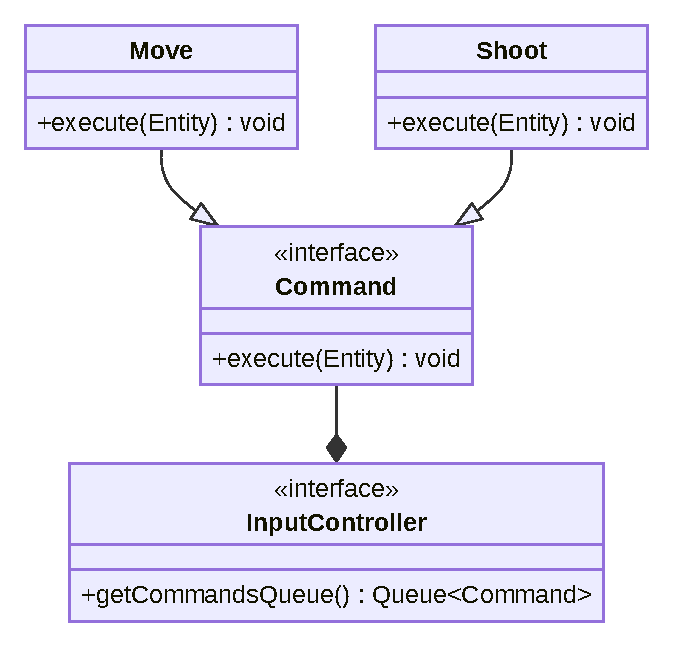
\includegraphics[scale=0.75]{img/CommandsUML}
\caption{Rappresentazione UML del pattern Command per la gestione dei comandi}
\label{img:command}
\end{figure}

\paragraph{Problema} Rendere riutilizzabili i comandi di gioco, separando la responsabilità di eseguirli dall’oggetto che li registra.

\paragraph{Soluzione} Il sistema di gestione dei comandi di gioco utilizza il \textit{Command pattern}. 
Questo pattern consente di incapsulare una richiesta, nel nostro caso un comando di input, in un oggetto. 
In questo modo il \textit{Command pattern} fornisce un livello di astrazione tra gli oggetti che triggerano azioni e quelli che le eseguono, 
riducendo la dipendenza tra questi oggetti.
La struttura del \textit{Command pattern} è composta da:
\begin{itemize}
\item \textbf{Command}: l'interfaccia che definisce l'operazione da eseguire. In questo caso rappresentato da \textit{Command}.
\item \textbf{Concrete Command}: classe che implementa l'interfaccia Command e specifica la logica di esecuzione per una determinata richiesta. In questo caso rappresentato da \textit{Move} e \textit{Shoot}.
\item \textbf{Receiver}: classe che contiene la logica vera e propria. I comandi gestiscono solo i dettagli di come una richiesta viene passata al \textit{receiver,} è infatti il \textit{receiver} che esegue il comando. In questo caso rappresentato dai diversi \textbf{Component}.
\item \textbf{Invoker}: classe che inizializza la richiesta. In questo caso rappresentato da \textbf{InputController + InputComponent}.
\end{itemize}
Altri vantaggi dell’utilizzo del \textit{Command pattern} sono la flessibilità e la riutilizzabilità. Infatti rende più facile l’aggiunta di nuovi comandi, la modifica di quelli esistenti o anche l’annullamento di comandi già eseguiti.

\subsubsection{Riuso di Input Controller}

\begin{figure}[H]
\centering{}
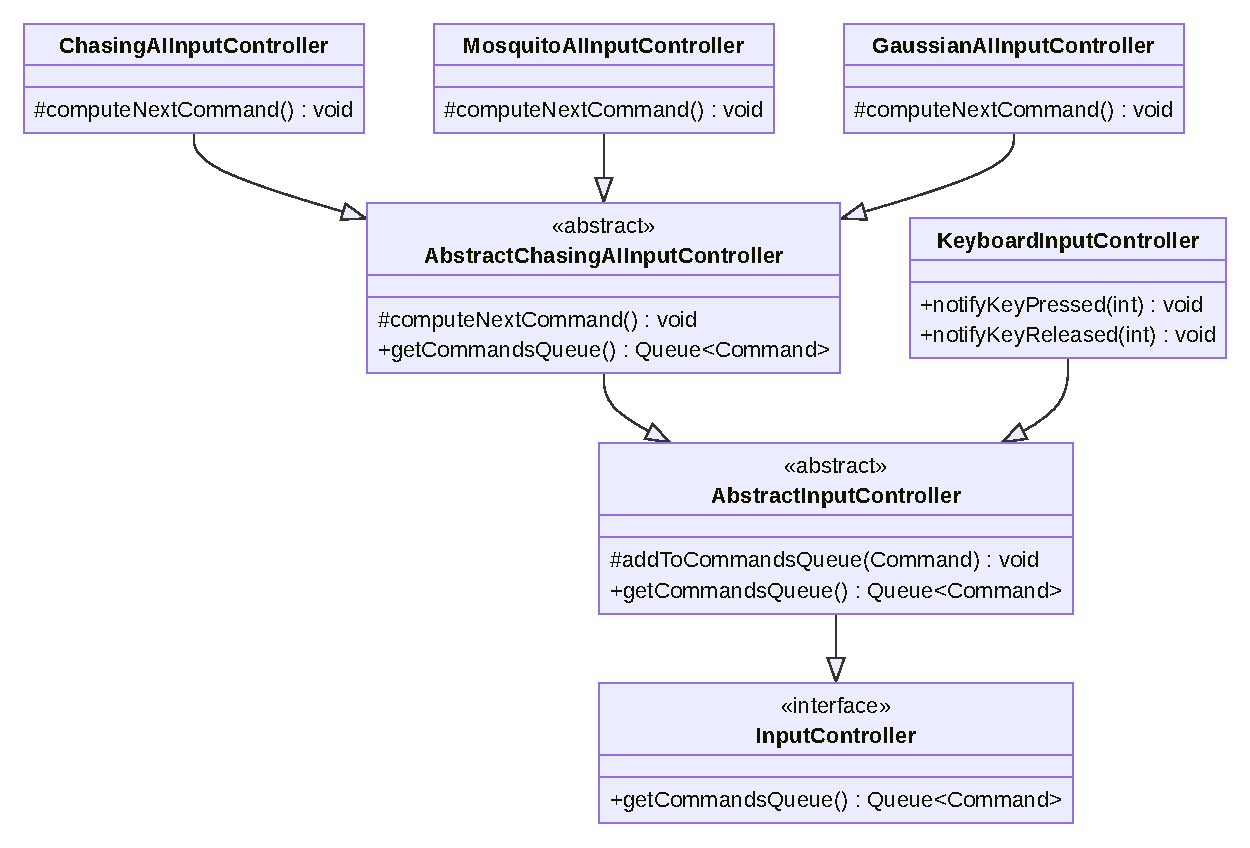
\includegraphics[scale=0.75]{img/InputControllerTemplateMethodUML}
\caption{Rappresentazione UML del pattern Template Method per il riuso di Input Controller}
\label{img:inputControllerTemplateMethod}
\end{figure}

\paragraph{Problema} Rendere riutilizzabili i comandi di gioco, separando la responsabilità di eseguirli dall’oggetto che li registra.

\paragraph{Soluzione} In \textit{AbstractInputController} viene data un’implementazione di default al metodo
\textit{getCommandsQueue()}, da questa classe astratta si possono costruire Input Controller 
come \textit{KeyboardInputController} che viene notificato ogni volta che un carattere da tastiera viene premuto
o rilasciato. Dato che un AI Input Controller non viene notificato da nessuna periferica, 
deve generare lui stesso i comandi da inserire nella \textit{commandsQueue}. 
Dato che diverse AI differiscono solamente per il metodo di generazione di comandi, è stato utilizzato il \textit{Template Method pattern}. 
\\
Nella classe \textit{AbstractChasingAIInputController} viene fatto l’override del metodo \textit{getCommandsQueue()} rendendolo il \textit{metodo di template} che, 
prima di ritornare la Commands Queue, chiama il metodo astratto \textit{computeNextCommand()}, 
il quale aggiunge in coda un comando generato seguendo l’algoritmo della data AI.

\subsubsection{Input Controller con molteplici stati}

\begin{figure}[H]
\centering{}
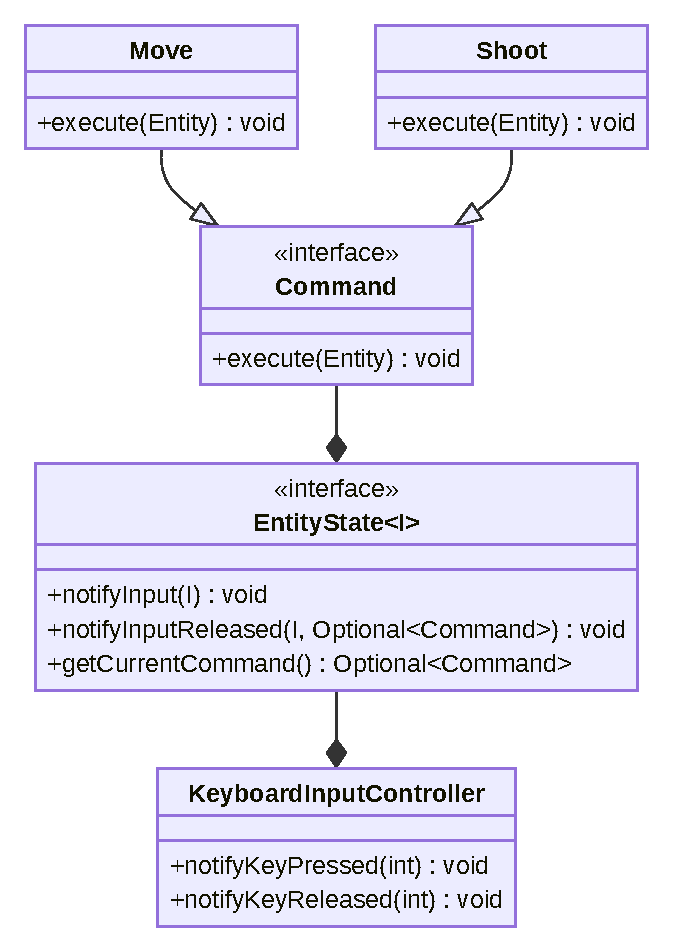
\includegraphics[scale=0.75]{img/EntityStateUML}
\caption{Rappresentazione UML del pattern State per la creazione di Input Controller con più FSM}
\label{img:inputControllerStatePattern}
\end{figure}

\paragraph{Problema} Rendere riutilizzabili i comandi di gioco, separando la responsabilità di eseguirli dall’oggetto che li registra.

\paragraph{Soluzione} Un player al momento presenta due \textit{macchine a stati finiti} (FSM): 
\textit{moveState} e \textit{shotState}. Ad ogni momento c'è un numero finito di stati in cui \textit{moveState} può stare: UP, DOWN, LEFT, RIGHT e STAY. 
Ad ognuno di questi stati corrisponde un comando (comportamento) diverso. \textit{moveState} può passare da uno stato ad un altro tramite regole dette \textit{transitions}, 
in questo caso le \textit{transitions} sono definite da un \textit{moveset} dove ad ogni input da tastiera corrisponde un comando. 
L'implementazione di questa FSM (e similmente anche per \textit{shotState}) è stata fatta utilizzando lo \textit{State pattern}, dove le implementazioni degli stati \textit{(Concrete States)} sono oggetti 
della classe \textit{Move} inizializzata con \textit{Directions} differenti, mentre il \textit{Context} è rappresentato da un implementazione di \textit{EntityState}. 
Grazie a questo pattern viene ridotta notevolmete la ripetizione di codice e semplificata l'aggiunta di ulteriori stati.
L'azione "sparare" è rappresentabile in quattro stati: UP, DOWN, LEFT, RIGHT; corrispondenti alla direzione del proitettile. Se "sparare" venisse trattato nella stessa FSM in cui viene gestito il movimento, per poter eseguire queste due azioni contemporaneamente, dovremmo duplicare il numero di stati.
Per risolvere questo problema vengono usate delle \textit{Concurrent State Machines}, ovvero due FSM che operano in maniera indipendente, in questo caso \textit{moveState} e \textit{shotState}.

\subsubsection{Gestione degli eventi di gioco}

\begin{figure}[H]
\centering{}
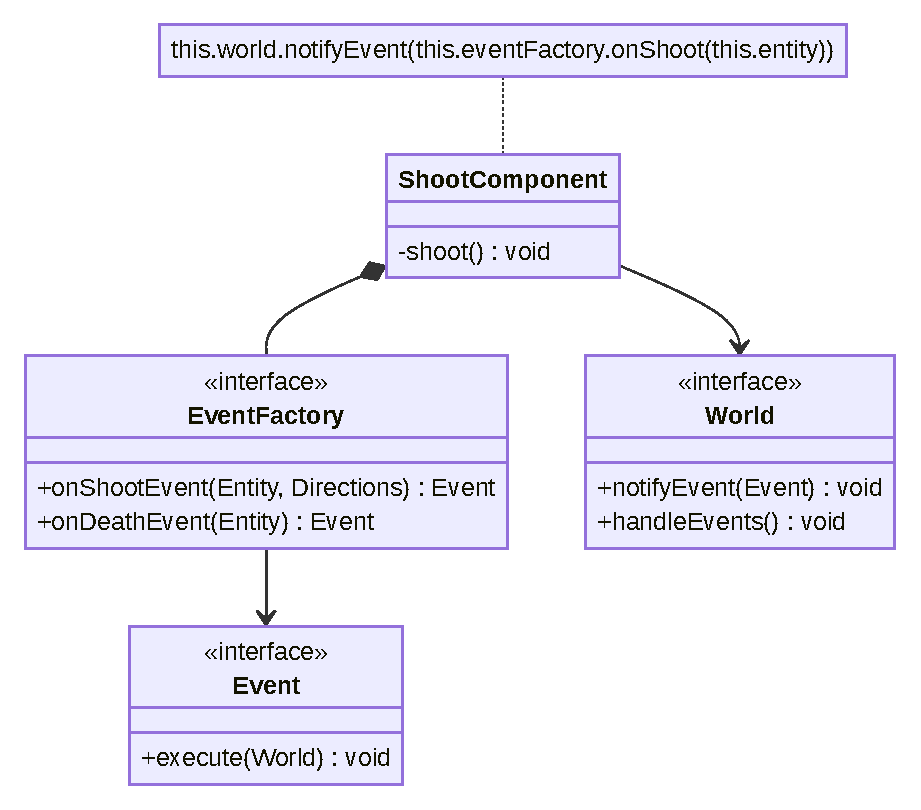
\includegraphics[scale=0.75]{img/EventsUML}
\caption{Rappresentazione UML della gestione degli eventi}
\label{img:eventsHandling}
\end{figure}

\paragraph{Problema} Dato che sono i Component a generare eventi, essi verrebbero generati quando viene chiamato il metodo \textit{update} di un component, quindi all’interno di un ciclo, incorrendo nel rischio di eccezioni \textit{“ConcurrentModificationException”}.

\paragraph{Soluzione} Per disaccoppiare l'evento generato da quando viene eseguito, utilizziamo il \textit{Pattern Event Queue}. 
Come descritto nel libro "Game Programming Patterns" di Robert Nystrom: \textit{"Una coda memorizza una serie di notifiche o richieste in ordine FIFO (First-In First-Out). 
Inviare una notifica aggiunge la richiesta alla coda e ritorna. Il "Request Processor" elabora quindi gli elementi nella coda in un secondo momento. 
Le richieste possono essere gestite direttamente o inoltrate ad altri oggetti. Questo disaccoppia il mittente dal destinatario sia staticamente che nel tempo"}
\footnote{\url{https://gameprogrammingpatterns.com/event-queue.html\#the-pattern}}.
\\
Prendiamo come esempio l'evento \textit{onShoot}. La gestione degli eventi è analoga anche per \textit{onPowerUp} e \textit{onDeath}. Quando uno ShootComponent vuole generare un proiettile, chiama il metodo notifyEvent(Event) del \textit{Request Processor} World, 
passandogli un evento come parametro. Questo evento viene aggiunto alla coda della Event Queue. Gli eventi possono essere generati tramite una \textit{Factory}.
\\
Al prossimo update del Game, verrà chiamato il metodo handleEvents() del World, che eseguirà ogni comando presente nella coda, e poi la pulirà.
\subsection*{Fiumanò Luca Oskari}

\subsubsection{Gestione delle Wave}

\begin{figure}[H]
\centering{}
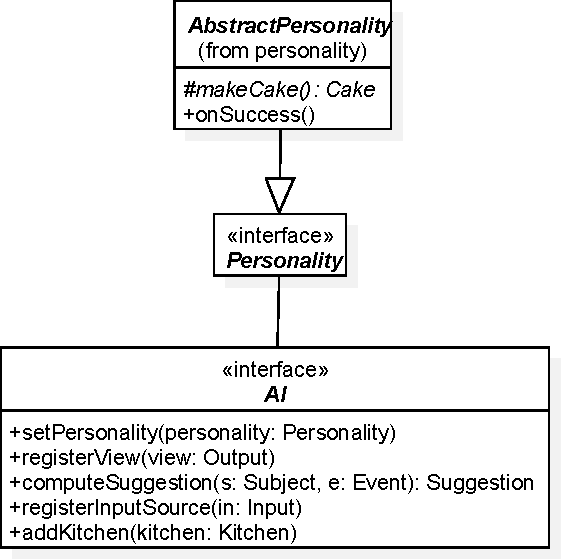
\includegraphics[width=\textwidth]{img/strategy}
\caption{Rappresentazione UML del pattern Factory per la gestione delle Wave}
\label{img:strategy}
\end{figure}

\paragraph{Problema} Esistono diversi tipi di Wave ognuna composta da nemici di vario tipo e numero.

\paragraph{Soluzione} Inizialmente per risolvere questo problema volevo utilizzare il \textit{Prototype} pattern creando una singola istanze per ogni tipo di nemico (prototipi) che sarebbero state clonate quando ritenute necessarie, inizialmente l’implementazione mi sembrava appropriata per risolvere il problema, ma non avevo preso in considerazione un problema fondamentale del pattern, infatti il metodo clone() che applicava il pattern non creava mai una nuova istanza ma passava solamente un riferimento del prototipo su cui era stato chiamato; questo causava diversi problemi, usando questo pattern i nemici avrebbero avuto tutti un riferimento agli stessi componenti questo causava ad esempio la condivisione di danno ricevuto tra tutti i nemici che avevano clonato lo stesso prototipo.
Ho capito quindi che sarebbe servito un pattern che creasse i diversi tipi di Wave formandole con istanze diverse di nemici; dopo un attenta ricerca la soluzione migliore mi è sembrata l’utilizzo di una \textit{Factory}. Così facendo mi sarei ritrovato nella condizione di poter creare un diverso tipo di wave con la sola chiamata di un metodo della \textit{Factory} senza incappare in errori di riferimenti comuni.

\subsubsection{Gestione delle Window indipendentemente dall'architettura grafica scelta}

\begin{figure}[H]
\centering{}
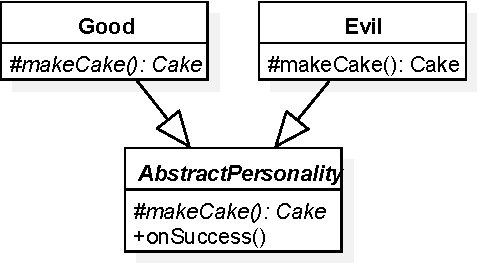
\includegraphics[width=\textwidth]{img/template}
\caption{Rappresentazione UML dell'applicazione del pattern Template Method alla Window}
\label{img:template}
\end{figure}

\paragraph{Problema} La gestione delle Window deve essere indipendente dall'architettura grafica scelta.

\paragraph{Soluzione} Per risolvere il problema ho deciso di utilizzare una classe astratta AbstractWindow che implementa il \textit{template method pattern} per definire come verranno create le scene. I template method sono \texttt{createGameScene()}, \texttt{createMenuScene()} e \texttt{createGameOverScene()} che utilizzano il metodo astratto \texttt{getSceneFactory()} che sarà implementato concretamente in una classe che estende AbstractWindow.

\subsubsection{Gestione delle diverse scene indipendentemente dall'architettura grafica scelta}

\begin{figure}[H]
\centering{}
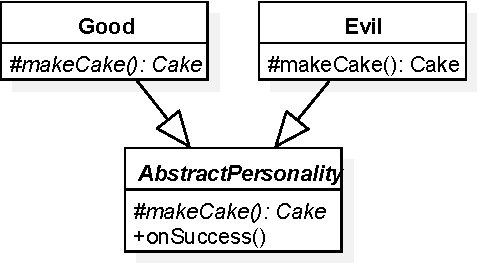
\includegraphics[width=\textwidth]{img/template}
\caption{Rappresentazione UML dell'applicazione del pattern FactoryMethod alla Scene}
\label{img:template}
\end{figure}

\paragraph{Problema} La gestione e creazione delle Scene deve essere indipendente dall'architettura grafica scelta.

\paragraph{Soluzione} Per venire a capo del problema ho deciso di utilizzare il \textit{pattern Factory} per delegare la creazione delle diverse scene in maniera indipendente dall'architettura grafica scelta; infatti se si volesse utilizzare una determinata architettura si dovrebbe creare una \textit{Factory} concreta per essa.

\subsubsection{Gestione di multipli PowerUp}

\begin{figure}[H]
\centering{}
% 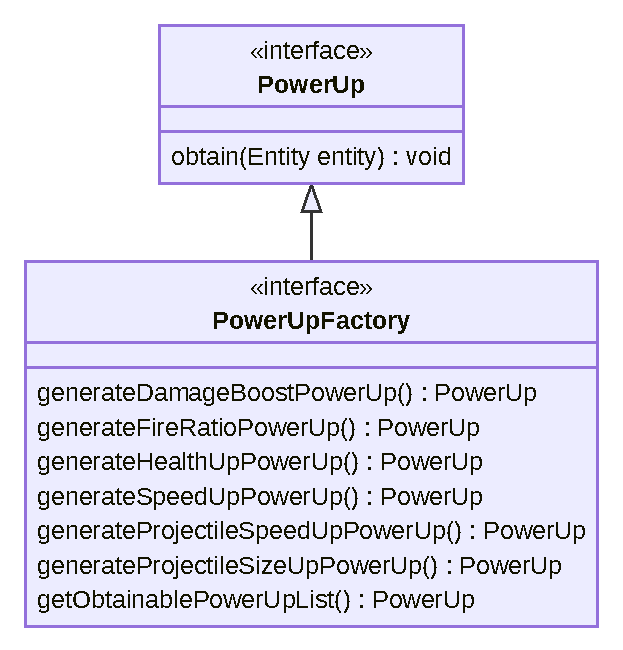
\includegraphics[width=\textwidth]{img/PowerUpUML}
\caption{Rappresentazione UML dell'applicazione del pattern Factory e Strategy ai PowerUp}
\label{img:observer}
\end{figure}

\paragraph{Problema} Il gioco deve implementare diversi tipi di PowerUp, ognuno che lavora su componenti diversi, che devono essere gestiti.

\paragraph{Soluzione} Dato che il nostro gioco doveva avere la possibilità di creare diversi tipi di PowerUp ognuno con comportamenti diversi ho deciso di utilizzare il \textit{Factory pattern} per sostituire la costruzione diretta dei PowerUp con delle appropriate chiamate alla \textit{Factory}. L'utilizzo del \textit{Factory method pattern} si è portato dietro un altro vantaggio la possibilità di aggiungere facilmente nuovi PowerUp.
Per risolvere il problema dei diversi comportamenti ho invece usato il pattern Strategy direttamente dentro la \textit{Factory} mediante il suo metodo privato \texttt{fromFunction()}.

\subsection*{Magnani Leonardo David Matteo}

\subsubsection{Getione delle entità}

\begin{figure}[H]
\centering{}
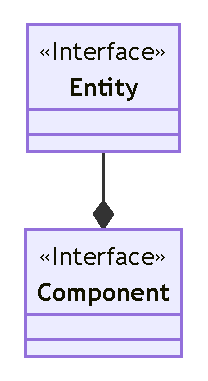
\includegraphics[width=.3\textwidth]{img/EntityComponentUML}
\caption{Rappresentazione UML dell'applicazione del Component Pattern alla enttità}
\end{figure}

\paragraph{Problema} La classe \texttt{Entity} copre più domini rompendo il \textit{Single Responsability Principle}.
Inoltre l'interfaccia \texttt{Entity} potrebbe avere numerose implementazioni in base al comportamento che li si vuole dare.
L'utilizzare la ereditarietà comporterebbe la creazione di molte sottoclassi con la conseguenza di ripetizione di codice.
Inoltre utilizzare l'ereditarietà multipla potrebbe portare numerosi problemi, come Deadly Diamond.

\paragraph{Soluzione} Il \textit{Component pattern} permette di creare dei componenti altamente riusabili e indipendenti.
Utilizzando il \textit{Component pattern}, quindi favorendo la composizione rispetto alla ereditarietà, si riesce a scaltare
molto velocementerent sul numero di entità.
Per descrivere il comportamento generale dell'entità li si vengono assegnati i componenti desiderati.
Dividendo il dominio e assegnando un dominio specifico ad un specifico componente viene rispettato il \textit{Single Responsability Principle}.
Questo comporta un migliore manutenibilità dovuta all'assenza di ripetizione di codice.\\
NOTA: La progettazione alla soluzione del problema è stata fatta in collaborazione con Cecchini Andrea.

\subsubsection{Comunicazione tra le componenti dell'entità}

\begin{figure}[H]
\centering{}
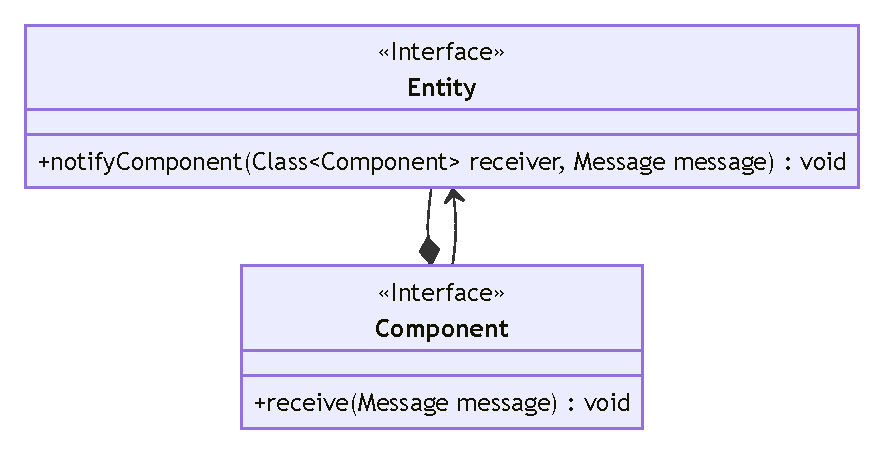
\includegraphics[width=\textwidth]{img/ComponentCommunicationUML}
\caption{Rappresentazione UML dell'applicazione del Mediator pattern per la comunicazione tra le componenti}
\end{figure}

\paragraph{Problema} I componenti hanno bisogno di comunicare tra di loro. Nel progetto:
\begin{itemize}
	\item InputComponent deve notificare il movimento da effettuare al PhysicsComponent.
	\item PhysicsComponent deve notificare il CollisionComponent della nuova posizione dopo il movimento.
	\item CollisionComponent deve notificare HealthComponent per indicare il danno ricevuto dalla collisione.
\end{itemize}
\paragraph{Soluzione} Il \textit{Mediator Pattern} è un modo efficace di gestire la comunicazione tra componenti
all'interno di un'entità. Utilizzando tale pattern, ciascun componente può inviare messaggi a un altro componente 
tramite la sua entità/mediatore. Ogni componente ha una referenza alla sua entità, consentendogli di inviare messaggi
a un componente specifico utilizzando il metodo \texttt{notifyComponent()}. Una volta ricevuto il messaggio, l'entità 
si occupa di passarlo al componente desiderato tramite il metodo \texttt{receive()}, consentendo così al componente ricevente 
di decidere come gestire il messaggio. Questo pattern offre la versatilità necessaria per gestire la comunicazione tra componenti 
in modo efficace e affidabile. \\
NOTA: La progettazione alla soluzione del problema è stata fatta in collaborazione con Cecchini Andrea.

\subsubsection{Creazione di collisioni con comportamenti diversi}

\begin{figure}[H]
\centering{}
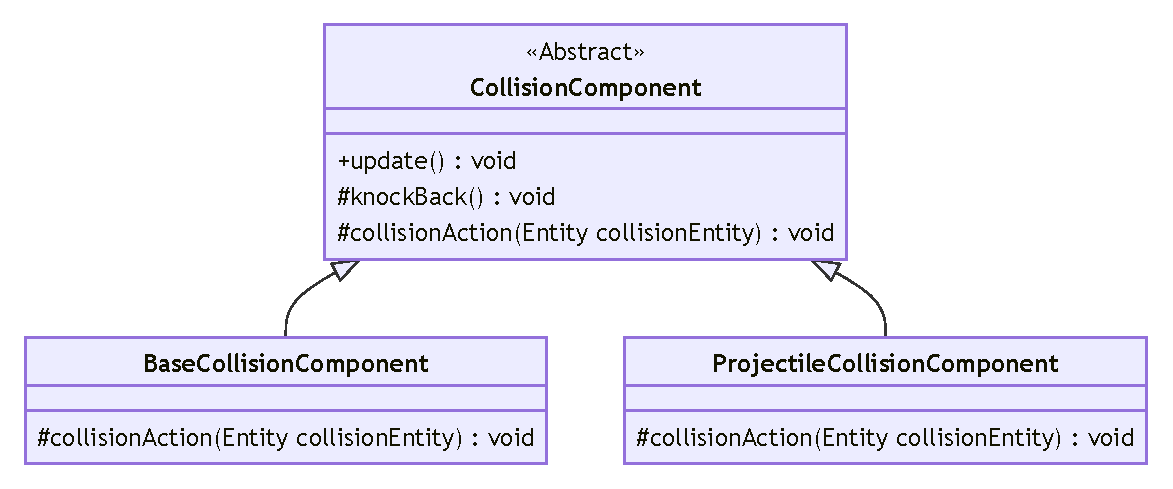
\includegraphics[width=\textwidth]{img/CollisionComponentUML}
\caption{Rappresentazione UML dell'applicazione del Template Method per la gestione di CollisionComponent con comportamenti diversi}
\end{figure}
	
\paragraph{Problema} Alcune entità devono agire in modo diverso in caso di collisione. Nel progetto, 
alcune entità perdono la vita in base al danno causato dalla collisione, mentre altre (i proiettili) si distruggono all'impatto.
\paragraph{Soluzione} Per gestire diverse entità che devono comportarsi in modo diverso in caso di collisione, nel progetto è 
stato utilizzato il \textit{Template Method pattern}. Il metodo template è \texttt{update()}, che chiama un metodo astratto \texttt{collisionAction()} 
per gestire il comportamento che l'entità deve prendere in caso di collisione, e un metodo protetto \texttt{knockback()} che gestisce il 
comportamento della collisione con entità rigide. In questo modo, si è creato un modo riutilizzabile e flessibile per gestire le 
collisioni tra entità che devono agire in modo diverso. \\
Il metodo \texttt{knockback()} anche se non utilizzato nell’implementazioni è stato messo per futura estendibilità.

\subsubsection{Creazione delle entità}

\begin{figure}[H]
\centering{}
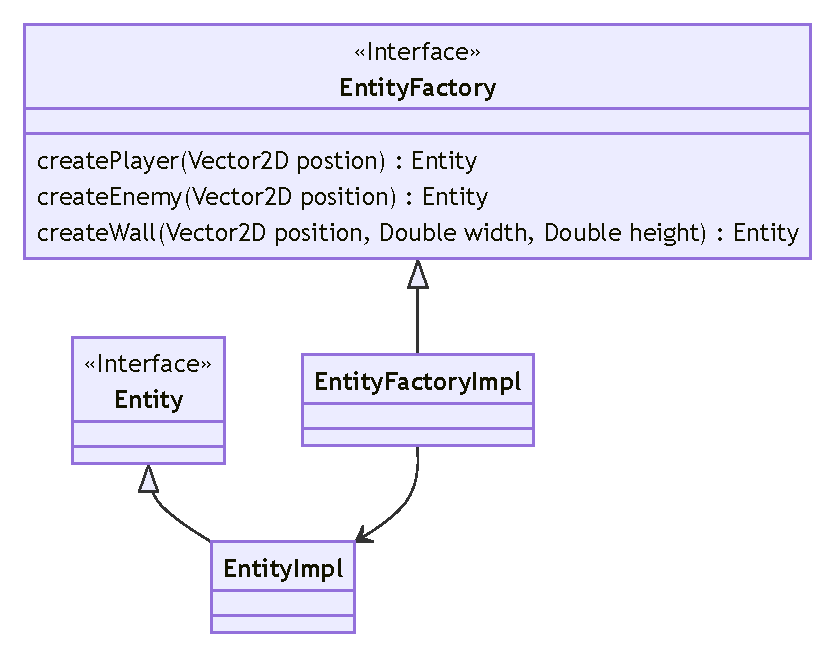
\includegraphics[width=\textwidth]{img/EntityFactoryUML.pdf}
\caption{Rappresentazione UML dell'applicazione del Factory Method per la creazione di diversi tipi di entità, 
\\NOTA: sono mostrate solo tre funzioni nella factory per rapprestazione}
\end{figure}
	
\paragraph{Problema} Ci possono essere più entità con componenti diversi e quindi comportamenti diversi.
\paragraph{Soluzione} Per la creazione di entità è stato utilizzato il \textit{Factory Method pattern}, è un modo semplice e flessibile 
per creare entità con componenti diversi e quindi comportamenti diversi. Ad esempio, una factory può creare un'entità che ha una 
fisica e collisione, oppure un’entità che abbia solo una collisione (come il muro di gioco). Una factory crea una superficie di 
abstracation per la creazione delle entità e nasconde la loro logica di implementazione. Tramite questo pattern, un codice chiamante può 
passare dei parametri specifici e ricevere un'istanza di un'entità pre-configurata. Questo significa che non è necessario scrivere il codice 
di creazione di un'entità in più posti, ma basta creare una factory una volta e passare i parametri a seconda dei casi d'uso.

\subsubsection{Riuso del codice delle personalità}

\begin{figure}[H]
\centering{}
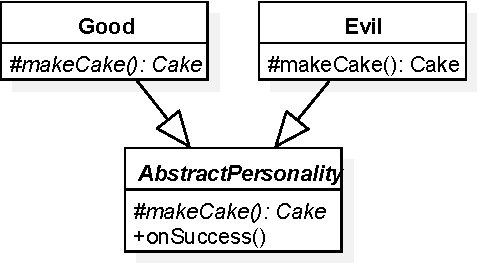
\includegraphics[width=\textwidth]{img/template}
\caption{Rappresentazione UML dell'applicazione del pattern Template Method alla gerarchia delle Personalità}
\label{img:template}
\end{figure}

\paragraph{Problema} In fase di sviluppo, sono state sviluppate due personalità, una buona ed una cattiva.
Quella buona restituisce sempre una torta vera, mentre quella cattiva restituisce sempre la
promessa di una torta che verrà in realtà disattesa.
Ci si è accorti che diverse personalità condividevano molto del comportamento,
portando a classi molto simili e a duplicazione.

\paragraph{Soluzione} Dato che le due personalità differiscono solo per il comportamento da effettuarsi in caso di percorso completato con successo,
è stato utilizzato il \textit{pattern template method} per massimizzare il riuso, come da \Cref{img:template}.
Il metodo template è \texttt{onSuccess()}, che chiama un metodo astratto e protetto
\texttt{makeCake()}.

\subsubsection{Gestione di output multipli}

\begin{figure}[H]
\centering{}
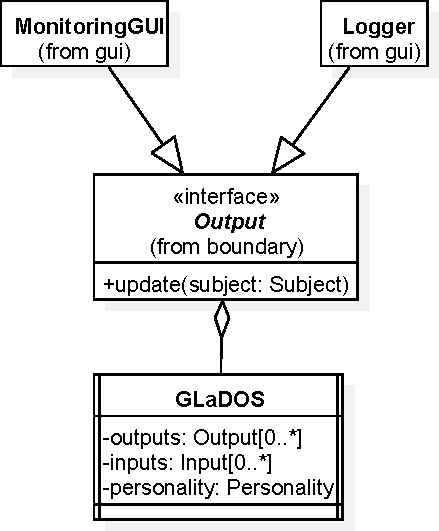
\includegraphics[width=.7\textwidth]{img/observer}
\caption{Il pattern Observer è usato per consentire a GLaDOS di informare tutti i sistemi di output in ascolto}
\label{img:observer}
\end{figure}

\paragraph{Problema} Il sistema deve supportare output multipli. In particolare, si richiede che vi sia un logger che stampa a terminale o su file,
e un'interfaccia grafica che mostri una rappresentazione grafica del sistema.

\paragraph{Soluzione} Dato che i due sistemi di reporting utilizzano le medesime informazioni, si è deciso di raggrupparli dietro l'interfaccia \texttt{Output}.
A questo punto, le due possibilità erano quelle di far sì che \texttt{GLaDOS} potesse pilotarle entrambe.
Invece di fare un sistema in cui questi output sono obbligatori e connessi, si è deciso di usare maggior flessibilità (anche in vista di future estensioni)
e di adottare una comunicazione uno-a-molti fra \texttt{GLaDOS} ed i sistemi di output.
La scelta è quindi ricaduta sul \textit{pattern Observer}: \texttt{GLaDOS} è observable, e le istanze di \texttt{Output} sono observer.
%
Il suo utilizzo è esemplificato in \Cref{img:observer}

\chapter{Sviluppo}
\section{Testing automatizzato}

Per effettuare i test abbiamo utilizzato JUnit 5.
\\I test che abbiamo effettuato sono:
\begin{itemize}
	\item \textbf{ShapeTest}, questa classe controlla le intersezioni tra i differenti Shape, assicurandosi che funzionino come previsto.
	\item \textbf{StopWatchTest}, questa classe verifica il funzionamento dello StopWatch nel caso in cui cerca di avviarlo quando già avviato oppure di fermarlo quando già fermato.
	\item \textbf{Vector2DTest}, questa classe verifica che le operazioni di Vector2D siano esatte.
	\item \textbf{GameEngineTest}, testati i getter del gameEngine, in modo tale da controllare che non ritornassero elementi nulli. E' stato controllato l'accesso ai metodi run e stop, in modo tale da verificare se venissero lanciate le giuste eccezioni quando il programmatore effettua errori di programmazione.
	\item \textbf{MessageTest}, in questa classe viene testato la messaggistica tra le componenti. Di preciso ho testato la comunicazione e ricevimento dei messaggi del PhysicsComponent e CollisionComponent
	\item \textbf{GameTest}, sono state testate le funzionalità basiche della classe Game, in particolare i vari getters, l'update e il metodo isOver(). Inoltre sono stati testati i metodi della factory di game, in modo da verificare che tali metodi ritornassero gli oggetti della classe Game con le caratteristiche volute
	\item \textbf{StateTest}, si testa l'implementazione della logica e dello stato della partita, in particolare 
        \begin{itemize}
    	    \item L'incremento del round e il suo relativo get.
            \item Controllo dello stato attuale della partita attraverso il metodo isOver. 
            \item Controllo dello stato della wave del round corrente
    	\end{itemize}
	\item \textbf{EntityTest}: questa classe verifica che si ottengano i componenti giusti dall’entità quando richiesti.
	\item \textbf{EventTest}, in questa classe vengono testati i vari tipi di eventi, controllando che vengano eseguiti dal World e non prima.
	\item \textbf{HealthComponentTest}, si testa il funzionamento del componente HealthComponent controllando specificatamente cosa succede quando si riceve un danno minore della vita attuale e cosa succede se si riceve un danno che porterebbe la vita sotto lo zero.
	\item \textbf{InputTest}, in questa classe viene testato l’input da testiera ec una delle AI.
	\item \textbf{PowerUpTest}, si testa il corretto funzionamento di tutti i possibili power up.
	\item \textbf{WaveTest}, in questa classe di test viene testato la corretta generazione di una wave controllando specificatamente la generazione di una wave basica e di una wave con boss, viene inoltre testato il la correttezza dell’aggiunta di un Entity alla wave.
	\item \textbf{WorldTest}, sono state testate funzioni basi come l'aggiunta e rimozione di entità, il metodo set e get dell'oggetto  Wave all'interno del mondo. Inoltre sono stati testati i metodi della factory di world, in modo da verificare che tali metodo ritornassero world con le caratteristiche volute
\end{itemize}
Dal punto di vista della grafica non sono stati svolti test automatizzati visto che la totalità della renderizzazione grafica è stata affidata al componente Canvas di JavaFX e al suo GraphicContext, risultavano quindi veramente minime le funzionalità da testare. Inoltre ciò che doveva essere visibile alla grafica veniva prelevato dal controller e altri eventuali test sarebbero stati solo ripetizioni di test già effettuati.



\section{Metodologia di lavoro}

Prima di cominciare con lo sviluppo abbiamo impostato l’architettura del gioco per avere delle solide fondamenta, iniziando con la definizione delle interfacce.
\\
La suddivisione iniziale del processo è stata fatta in maniera adeguata, consentendoci di lavorare parallelamente; riunendoci solo quando era necessario interlacciare le diverse implementazioni o per discutere su eventuali aggiunte.
\\
Abbiamo deciso di utilizzare il DVCS con il semplice approccio spiegato in classe, difatti dopo la creazione del repository ognuno di noi ne ha fatto un clone per lavorarci in autonomia condividendo le aggiunte mediante pull e push.

\subsection*{Cecchini Andrea}
In autonomia mi sono occupati di:
\begin{itemize}
	\item GameEngine e GameLoop (package t2sgame.core.engine)
	\item Implementazione del gioco (package t2sgame.game)
	\item Implementazione del mondo di gioco (package t2sgame.game.model)
	\item Implementazione della logica di gioco (package t2sgame.game.logics)
\end{itemize}
In collaborazione mi sono occupato:
\begin{itemize}
	\item Con Leonardo Magnani:
		\begin{itemize}
			\item Gestione delle collisioni: mi sono occupato di trovare un modo flessibile e mantenibile per gestire la collisione fra forme di tipo diverso.
			\item Gestione dei componenti.
			\item Gestione della messagistica.
		\end{itemize}
\end{itemize}
\subsection*{Nicolò D'Addabbo}
In autonomia mi sono occupato di:
\begin{itemize}
\item Input Component (in t2sgame.game.ecs.impl)
\item Gestione degli input da periferica (package t2sgame.input)
\item AI (package t2sgame.input)
\item Comandi di gioco (package t2sgame.input)
\item Gestione degli eventi (Event ed EventFactory in t2sgame.game.logics e metodi notifyEvent e handleEvent in World)
\end{itemize}

\subsection*{Magnani Leonardo David Matteo}
In autonomia mi sono occupato di:
\begin{itemize}
\item Le entità di gioco (Entity in t2sgame.game.ecs)
\item Alcune componenti delle entità (DamageComponent e ShootComponent in t2sgame.game.ecs.impl)
\item La fisica del gioco (PhysicsComponent in t2sgame.game.ecs.impl, Vector2D in  t2sgame.common)
\item Le implemtazioni delle collisioni (BaseCollisionComponent e ProjectileCollisionComponent in t2sgame.game.ecs.impl, Circle e Rectangle in t2sgame.common.shapes)
\item Uno stopwatch per la gestione del tempo trascorso (StopWatch in t2sgame.common)
\end{itemize}

\section{Note di sviluppo}
\subsection*{Cecchini Andrea}
\subsubsection*{Utilizzo di Stream}
L'uso di streams pervade la maggior parte del codice.
Il seguente è solo un esempio: 
\\
\url{https://github.com/nicolodaddabbo/OOP22-t2s-game/blob/6dc6e41a127a2c02e07ca14e6265c07ac3afeeb1/src/main/java/it/unibo/t2sgame/core/engine/impl/GameEngineImpl.java#L115-L119}

\subsubsection*{Creazione di interfacce funzionali}
Esempio di una classe funzionale utilizzata per incapsulare messaggi tra componenti:
\\
\url{https://github.com/nicolodaddabbo/OOP22-t2s-game/blob/a2aae31b62e6f41b9cc2d0ee80a388e56f2b42db/src/main/java/it/unibo/t2sgame/game/ecs/api/Message.java#L3-L15}
\subsubsection*{Utilizzo di Lambda e Method references}
Sono numerosi gli utilizzi di lambda e method references. In seguito alcuni esempi: 
\\
\url{https://github.com/nicolodaddabbo/OOP22-t2s-game/blob/6dc6e41a127a2c02e07ca14e6265c07ac3afeeb1/src/main/java/it/unibo/t2sgame/core/engine/impl/GameEngineImpl.java#L145-L155}


\subsection*{Nicolò D'Addabbo}
\subsubsection*{Utilizzo di Stream, lambda expression e method reference}
Usate molto spesso in vari punti del progetto:
\begin{itemize}
	\item Permalink: \url{https://github.com/nicolodaddabbo/OOP22-t2s-game/blob/d1453f9e5f56d2cdfec21561311304a309e99ed9/src/main/java/it/unibo/t2sgame/game/logics/impl/EventFactoryImpl.java#L37}
	\item Permalink: \url{https://github.com/nicolodaddabbo/OOP22-t2s-game/blob/d1453f9e5f56d2cdfec21561311304a309e99ed9/src/main/java/it/unibo/t2sgame/input/api/AbstractChasingAIInputController.java#L45-L48}
	\item Permalink: \url{https://github.com/nicolodaddabbo/OOP22-t2s-game/blob/d1453f9e5f56d2cdfec21561311304a309e99ed9/src/main/java/it/unibo/t2sgame/input/api/AbstractChasingAIInputController.java#L45-L48}
\end{itemize}
\subsubsection*{Classe con Generics}
\begin{itemize}
	\item Permalink: \url{https://github.com/nicolodaddabbo/OOP22-t2s-game/blob/d1453f9e5f56d2cdfec21561311304a309e99ed9/src/main/java/it/unibo/t2sgame/input/impl/EntityStateImpl.java#L14}
\end{itemize}

\subsection*{Magnani Leonardo David Matteo}
\begin{itemize}
	\item Utilizzo di stream, optional, method reference e metodo generico  \\
	Permalink: \url{https://github.com/nicolodaddabbo/OOP22-t2s-game/blob/48fe160af0c4cdbfbf7fe791b784f6f4ad7b185e/src/main/java/it/unibo/t2sgame/game/ecs/impl/EntityImpl.java#L46-L51}
	\item Utilizzo di stream, optional, lamda e metodo generico \\
	Permalink: \url{https://github.com/nicolodaddabbo/OOP22-t2s-game/blob/48fe160af0c4cdbfbf7fe791b784f6f4ad7b185e/src/main/java/it/unibo/t2sgame/game/ecs/impl/EntityImpl.java#L69-L71}
\end{itemize}

\chapter{Commenti finali}

\section{Autovalutazione e lavori futuri}
\subsection*{Andrea Cecchini}
Sono  contento dell'opportunità avuta nel realizzare questo progretto.
\\
Per quanto riguarda il lavoro in gruppo, sono molto soddisfatto del coordinamento che vi è stato.
Lo scambio di opinioni e di idee è una delle caratteristiche fondamentali che rappresenta il nostro gruppo.
\\
Questo progetto mi ha dato la possibilità di sperimentare moltissimo sul scrivere codice "pulito" e "riusabile".
Nonostante l'esperienza nello sviluppo di un gioco, sono abbastanza contento del risultato.
Ritengo comunque che ci siano parti da migliorare e come esercizio, una volta effettuata la consegna, avrò la possibilità di imparare ancora.

\subsection*{Nicolò D'Addabbo}
Sono soddisfatto del nostro progetto, che è stato un ottimo esercizio di lavoro di gruppo. Abbiamo collaborato in maniera efficace grazie a una buona fase di analisi, che è stata fondamentale per individuare quali problemi risolvere e come affrontarli. Questo progetto mi ha permesso di sviluppare abilità che possono essere applicate a progetti futuri, come la gestione del codice in gruppo ed una buona organizzazione del lavoro.
Ho lavorato alla parte Model e ho collaborato al Controller. Purtroppo non ho avuto la possibilità di approfondire JavaFX, che mi sarebbe interessato molto, poiché non ho avuto parti di View.

\subsection*{Magnani Leonardo David Matteo}
Sono soddisfatto del risultato finale considerando il tempo limitato a disposizione. 
La buona analisi effettuata prima dello sviluppo ha permesso di creare una solida base per il progetto. 
Nonostante alcune parti siano state riscritte durante la fase di sviluppo per migliorare il codice, l'architettura iniziale è rimasta intatta. 
Tuttavia, a causa di impegni accademici e del tempo limitato, non ho avuto la possibilità di apportare miglioramenti a certe parti del mio lavoro. 
Un'area di miglioramento potrebbe essere la gestione delle collisioni a cui ero molto interessato a fare efficientemente.
Anche se questo progetto mi ha permesso di acquisire competenze organizzative e architetturali e di mettere alla prova le mie capacità come ingegnere, 
personalmente ritengo che non sia il progetto giusto per me da portare avanti in futuro.

\appendix
\chapter{Guida utente}

Quando viene fatto partire l'applicativo ci si ritroverà in una scena con due bottoni:
\begin{itemize}
    \item \textbf{Single Player}: Versione del gioco in cui il giocatore è solo contro le ondate di nemici.
    \item \textbf{With Companion}: Versione del gioco semplificata in cui il giocatore è aiutato da un Companion (una semplice IA, che attacca i nemici) 
\end{itemize}

I comandi di gioco sono i seguenti:
\begin{itemize}
    \item \textbf{ESC} (Escape): chiude l'applicazione
    \item \textbf{W}: Movimento verso l'alto.
    \item \textbf{A}: Movimento verso sinistra.
    \item \textbf{S}: Movimento verso il basso.
    \item \textbf{D}: movimento verso destra
    \item \textbf{↑} (Up Arrow): sparo verso l'alto.
    \item \textbf{↓} (Down Arrow): sparo verso il basso.
    \item \textbf{←} (Left Arrow): sparo verso sinistra.
    \item \textbf{→}(Right Arrow): sparo verso destra.
\end{itemize}

\bibliographystyle{alpha}
\bibliography{13-template}
\end{document}
